\documentclass{article}
\usepackage{graphicx} % Required for inserting images
\usepackage{amsmath}
\usepackage{amssymb}
\usepackage{enumerate}
\usepackage[margin=1in]{geometry}
\usepackage{tcolorbox}
\usepackage{bm}
\usepackage{graphicx}


\usepackage{listings}
% Define colors for the code
\definecolor{codegreen}{rgb}{0,0.6,0}
\definecolor{codegray}{rgb}{0.5,0.5,0.5}
\definecolor{codepurple}{rgb}{0.58,0,0.82}
\definecolor{backcolor}{rgb}{0.95,0.95,0.92}

% Configure lstlisting for Python code
\lstdefinestyle{pythonstyle}{
    backgroundcolor=\color{backcolor},
    commentstyle=\color{codegreen},
    keywordstyle=\color{blue},
    numberstyle=\tiny\color{codegray},
    stringstyle=\color{codepurple},
    basicstyle=\ttfamily\footnotesize,
    breakatwhitespace=false,
    breaklines=true,
    captionpos=b,
    keepspaces=true,
    numbers=left,
    numbersep=5pt,
    showspaces=false,
    showstringspaces=false,
    showtabs=false,
    tabsize=4
}

\lstset{style=pythonstyle}


\newcommand{\mydivider}{\vspace{1em}\hrule\vspace{1em}}
\newcommand{\mypart}[2]{\noindent{\textbf{[#1] point(s) --- #2:}}}
\newcommand{\programming}{\textcolor{blue}{This is a programming exercise. See \texttt{hw5.ipynb}}}


\newcommand{\bfx}{\mathbf{x}}
\newcommand{\bfX}{\mathbf{X}}
\newcommand{\bfw}{\mathbf{w}}
\newcommand{\bfb}{\mathbf{b}}
\newcommand{\bfW}{\mathbf{W}}

%%% BEGIN MACROS
% type your macros here
%%% END MACROS


\title{CS 577 --- Deep Learning --- Homework 5}
\author{}
\date{}

\begin{document}

\maketitle
\textbf{Read these instructions carefully}:
\begin{itemize}
  \item
In the \LaTeX~source code, type your answer in between
``\verb|%%% BEGIN ANSWER|'' and
``\verb|%%% END ANSWER|''.
        For advanced \LaTeX users,
        you can use your custom macros if you wish
        by placing them
        between
``\verb|%%% BEGIN MACROS|'' and
``\verb|%%% END MACROS|'' in the header.
        Do not modify anything else.




  \item Turn in both your \verb|.tex| file and the generated \verb|.pdf| file.
\end{itemize}



\section{The transformer module}

In homework 3 and 4, we investigated computation for a simple attention model,
where each data  point
\(\bfX^{(i)}\)
is itself a \emph{collection} of \(C\) vectors (for concreteness, take \(C = 32\)).
Namely, we write
\(\bfX^{(i)}\) as a matrix whose \(c\)-th column is \(\bfx^{(i,c)}\), i.e.,

\[
\bfX^{(i)}
=
\begin{bmatrix}
\bfx^{(i,1)} & \cdots & \bfx^{(i,C)}
\end{bmatrix} \in \mathbb{R}^{d \times C} \quad \text{is a } d \times C \text{ matrix}
\]
You can think of the \(\bfx^{(i,j)}\)'s for each \(j = 1,\dots, C\) as the ``word embedding'' for some sentence of length \(C\).
We say that \(\bfX^{(i)}\) is a ``sequence''.

\vspace{1em}

In the code, we will name

\begin{itemize}
  \item

\(C\) as \texttt{n\_context}

  \item
\(d\) as \texttt{n\_features}

  \item
\(n\) as \texttt{n\_samples}, which denotes the mini-batch size \(\bfX^{(1)},\dots, \bfX^{(n)}\).

        
\end{itemize}



\textbf{The transformer module}
 that we consider in this homework is composed of a \emph{self-attention} submodule followed by a
\emph{multilayer perceptron} submodule with 1-hidden layer.
For simplicity, we focus on these two submodules, leaving aside for now dropout, layer norm, etc.
Both of these submodules will have parameters. We will refer to these parameters as
\(
\theta^{(\texttt{att})}
\)
and
\(
\theta^{(\texttt{mlp})}
\)
respectively.

\vspace{1em}


\textbf{The self-attention submodule} has parameters
\[
\theta^{(\texttt{att})} = [ \bfW^{(Q)}, \bfW^{(K)}, \bfW^{(V)}]
\qquad
\mbox{
  (``\(Q\), \(K\), \(V\)''
  stands for
  ``query'',
  ``key'',
  ``value'', respectively)
}
\]
where
\[
  \bfW^{(Q)} \text{ and } \bfW^{(K)}
  \text{ and  }
\bfW^{(V)} \in \mathbb{R}^{d \times d}.
\]

Here are the main changes compared to the previous homeworks
\begin{itemize}
  \item  We assume \(q = d\) for simplicity. In this homework, there is no separate \texttt{n\_reduced}.



  \item

In previous homeworks, we had \(\bfW^{(1)}\) instead of \(\bfW^{(Q)}\), and had \(\bfW^{(2)}\) instead of \(\bfW^{(K)}\).


  \item
        In previous homeworks, we had \(\bfw^{(3)}\) which was a vector.
In this homework, we have       that
 \(\bfW^{(V)}\) is a \(d \times d\) matrix.
\end{itemize}

In this homework, our self-attention submodule
is ``\textbf{seq-2-seq}'', i.e., it
maps the sequence \(\bfX^{(i)}\) to another sequence \(\texttt{attention}(\bfX^{(i)}; \theta)\):

\[
\texttt{attention}(\bfX^{(i)} ; \theta)
:=
\bfW^{(V) \top}
\bfX^{(i)}
\mathrm{softmax} \left( \bfX^{(i)\top} \bfW^{(K)\top } \bfW^{(Q)} \bfX^{(i)} \right)
\in \mathbb{R}^{d \times C}.
\]
Note that
\begin{itemize}
  \item
\(\mathrm{softmax} \left( \bfX^{(i)\top} \bfW^{(K)\top } \bfW^{(Q)} \bfX^{(i)} \right)\) is a \(C\)-by-\(C\) matrix.

  \item
        \(
\texttt{Attention}(\bfX^{(i)} ; \theta)
        \)
        has the same shape as
        \(
\bfX^{(i)}
        \)

\end{itemize}


\vspace{1em}




The \textbf{MLP submodule} has a single hidden layer and the following parameters:
\[
\theta^{(\texttt{mlp})} = [\bfW^{(H)}, \bfb^{(H)}, \bfW^{(\text{O})}, \bfb^{(\text{O})}]
\qquad
\mbox{
  (``\(H\), \(O\)''
  stands for ``hidden'' and ``output'', respectively)
}
\]
where
\[
\bfW^{(H)} \in \mathbb{R}^{d \times h}, \quad \bfb^{(H)} \in \mathbb{R}^{h}, \quad \bfW^{(\text{O})} \in \mathbb{R}^{h \times d}, \quad \text{and} \quad \bfb^{(\text{O})} \in \mathbb{R}^d.
\]
The hidden-layer activation is computed as
   \(     \mathbf{H} = \mathrm{relu}\left(\bfW^{(H)\top}\bfX^{(i)}
      + \bfb^{(H)}\right) \in \mathbb{R}^{h \times C}
\) and the output
   \[
     \mathtt{MLP}(\bfX^{(i)}; \theta^{(\texttt{mlp})})
     =
     \bfW^{(O)\top} \mathbf{H} + \bfb^{(O)}
     \in \mathbb{R}^{d \times C}
   \]
   Putting both submodules together,  we have the transformer block:
\[
\texttt{TransformerBlock}(\bfX^{(i)} \, ; \, \theta^{(\mathtt{att})}, \theta^{(\mathtt{mlp})}) := \texttt{MLP}(\texttt{Attention}(\bfX^{(i)}; \theta^{(\texttt{att})}) \, ; \, \theta^{(\texttt{mlp})})
\]
The above can be implemented (vectorizing over a batch \(\bfX^{(1)},\dots, \bfX^{(n)}\)) as follows:




\begin{lstlisting}[language=Python]
# IMPORTANT: the batch data tensor has shape (n_samples, n_context, n_features)
#
class SingleHeadAttention:
    def __init__(self, n_features):
        self.Wq = ag.Tensor(np.random.randn(n_features, n_features), label="Wq")
        self.Wk = ag.Tensor(np.random.randn(n_features, n_features), label="Wk")
        self.Wv = ag.Tensor(np.random.randn(n_features, n_features), label="Wv")
    def __call__(self, Xin):
        Queries = Xin @ self.Wq
        Keys = Xin @ self.Wk
        KQ = (Keys @ ag.moveaxis(Queries, 1,2))
        expKQ = ag.exp(KQ)
        softmaxKQ = expKQ / ag.sum(expKQ, axis=1, keepdims=True)
        Xout = ag.moveaxis(ag.moveaxis(Xin,1,2) @ softmaxKQ, 1,2) @ self.Wv
        return Xout

class MLP:
    def __init__(self, n_features, n_hidden):
        self.Wh = ag.Tensor(np.random.randn(n_features, n_hidden), label="Wh")
        self.bh = ag.Tensor(np.random.randn(n_hidden), label="bh")
        self.wo = ag.Tensor(np.random.randn(n_hidden, n_features), label="Wo")
        self.bo = ag.Tensor(np.random.randn(n_features), label="bo")

    def __call__(self, Xin):
        hidden = ag.relu((Xin @ self.Wh) + self.bh)
        return hidden @ self.wo + self.bo

class TransformerBlock:
    def __init__(self, n_features, n_hidden):
        self.att = SingleHeadAttention(n_features)
        self.mlp = MLP(n_features, n_hidden)
    def __call__(self, Xin):
        return self.mlp(self.att(Xin))
\end{lstlisting}


\newpage

\mypart{5}{part a}

\programming



\mydivider

\mypart{5}{part b}

Explain your answer from part a.

\begin{tcolorbox}
\textbf{Answer: }


%%% BEGIN ANSWER
% type your answer here
Firstly, the code calculates the \textbf{binary cross-entropy loss between the model’s output and the target} labels:

\[
\text{loss} = \text{nn.BinaryCrossEntropyLoss()}(\text{att}(X)[:, 3, 0], y)
\]

Here, the model's output is defined as \(\text{att}(X)[:, 3, 0]\), and \(y\) represents the true label. After calculating the loss, the gradient of the loss with respect to the model's parameters is computed with \(\text{loss.backward()}\) to \textbf{facilitate backpropagation.} \\
I selected the last element of the 3rd row of the output tensor, \(\text{att}(X)[:, 3, 0]\), as the model's output because the last row in each column represents an \textbf{accumulated summary} of information from all previous rows.
Finally, the second and third column of output are zeros because Wv have zero values in these columns, then any projection along those columns will yield zero values.
%%% END ANSWER

\end{tcolorbox}

\begin{figure}[h] 
    \centering
    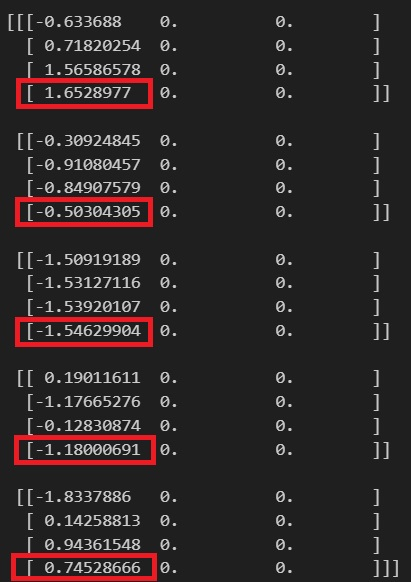
\includegraphics[width=0.5\linewidth]{att_result.jpg}  
    \caption{Output of the attention, in red the accumulated summary of information from all previous rows}
    \label{fig:your_label}
\end{figure}

\mydivider

\mypart{10}{part c}

Given that a single \texttt{matmul} between matrices of shape \((a,b)\) and \((b,c)\)
requires \(O(abc)\) floating point operations (FLOPs), compute the number of FLOPs required to compute one forward pass of the \texttt{TransformerBlock}
on an input tensor of shape \((n, C,d)\).
Give your answer in terms of big-O notation involving the quantities \(n,C,d\) and \(h\).


\begin{tcolorbox}
\textbf{Answer: }

%%% BEGIN ANSWER
To calculate the computational complexity for a forward pass through the \texttt{TransformerBlock}, given an input tensor of shape \((n, C, d)\), where:

\begin{itemize}
    \item \(n\) is the number of samples in the batch.
    \item \(C\) is the sequence length or context size.
    \item \(d\) is the input feature dimension.
    \item \(h\) is the hidden dimension size used in the \texttt{MLP} component.
\end{itemize}

The \texttt{TransformerBlock} consists of two main parts:
\begin{itemize}
    \item A \texttt{SingleHeadAttention} layer.
    \item An \texttt{MLP} layer.
\end{itemize}

Therefore, the total FLOPs for the \texttt{TransformerBlock} can be calculated as the \textbf{sum of the FLOPs} for the \texttt{SingleHeadAttention} and \texttt{MLP} layers.

\section*{1. FLOPs for the SingleHeadAttention Layer}

In the \texttt{SingleHeadAttention} layer:
\begin{itemize}
    \item \(\texttt{Wq}\), \(\texttt{Wk}\), and \(\texttt{Wv}\) are weight matrices of shape \((d, d)\).
    \item The input tensor \(\texttt{Xin}\) has a shape \((n, C, d)\).
\end{itemize}

\textbf{Steps and FLOPs in SingleHeadAttention:}
\begin{itemize}
    \item The input \(\texttt{Xin}\) is projected to Queries, Keys, and Values by multiplying with \(\texttt{Wq}\), \(\texttt{Wk}\), and \(\texttt{Wv}\).
    \item Each of these multiplications has a complexity of \(O(n \cdot C \cdot d^2)\), as the input \((n, C, d)\) is multiplied by a weight matrix of \((d, d)\).
    \item Since there are three projections (for \(\texttt{Wq}\), \(\texttt{Wk}\), and \(\texttt{Wv}\)), the total FLOPs for this step is:
    \[
    3 \cdot O(n \cdot C \cdot d^2) = O(n \cdot C \cdot d^2)
    \]
\end{itemize}

\textbf{Attention Score Calculation (Dot Product between Keys and Queries):}
\begin{itemize}
    \item After projecting Keys and Queries, they have shapes \((n, C, d)\).
    \item To calculate the attention scores, the dot product of Keys and Queries (with one axis moved) results in a matrix of shape \((n, C, C)\).
    \item This operation has a complexity of \(O(n \cdot C^2 \cdot d)\), as we are performing \(C \times C\) matrix multiplications for each sample and each feature dimension.
\end{itemize}

\end{tcolorbox}
\newpage
\begin{tcolorbox}

\textbf{Softmax Normalization:}
\begin{itemize}
    \item The softmax normalization over the attention scores has a complexity of \(O(n \cdot C^2)\), as it’s applied across the sequence length for each sample.
\end{itemize}

\textbf{Weighted Sum of Values:}
\begin{itemize}
    \item Finally, we compute the weighted sum of Values using the attention weights, resulting in an output shape of \((n, C, d)\).
    \item This operation also has a complexity of \(O(n \cdot C^2 \cdot d)\), as it involves matrix multiplications between the attention weights \((n, C, C)\) and Values \((n, C, d)\).
\end{itemize}


\textbf{Total FLOPs for SingleHeadAttention:}
Adding all these terms together, we get:
\[
O(n \cdot C \cdot d^2) + O(n \cdot C^2 \cdot d) + O(n \cdot C^2) + O(n \cdot C^2 \cdot d) = O(n \cdot C \cdot d^2 + n \cdot C^2 \cdot d)
\]

\section*{2. FLOPs for the MLP Layer}

In the \texttt{MLP} layer:
\begin{itemize}
    \item \(\texttt{Wh}\) (the first weight matrix) has a shape of \((d, h)\).
    \item \(\texttt{Wo}\) (the second weight matrix) has a shape of \((h, d)\).
    \item The input to the \texttt{MLP} layer has shape \((n, C, d)\).
\end{itemize}

\textbf{First Linear Transformation:}
\begin{itemize}
    \item The input \((n, C, d)\) is multiplied by \(\texttt{Wh}\) (of shape \((d, h)\)) to produce a hidden representation of shape \((n, C, h)\).
    \item This matrix multiplication has a complexity of \(O(n \cdot C \cdot d \cdot h)\).
\end{itemize}

\textbf{ReLU Activation:}
\begin{itemize}
    \item The ReLU activation function is applied element-wise on \((n, C, h)\), with a complexity of \(O(n \cdot C \cdot h)\).
\end{itemize}

\textbf{Second Linear Transformation:}
\begin{itemize}
    \item The hidden representation \((n, C, h)\) is multiplied by \(\texttt{Wo}\) (of shape \((h, d)\)) to produce an output of shape \((n, C, d)\).
    \item This matrix multiplication has a complexity of \(O(n \cdot C \cdot h \cdot d)\).
\end{itemize}

\textbf{Total FLOPs for MLP:}
Adding up the terms, we get:
\[
O(n \cdot C \cdot d \cdot h) 
\]

\section*{Total FLOPs for the TransformerBlock}

Now, combining the FLOPs from \texttt{SingleHeadAttention} and \texttt{MLP}, we get the total FLOPs for one forward pass through the \texttt{TransformerBlock}:
\[
O(n \cdot C \cdot d^2) + O(n \cdot C^2 \cdot d) + O(n \cdot C \cdot d \cdot h)
\]
\[
O(n \cdot C \cdot d^2 + n \cdot C^2 \cdot d + n \cdot C \cdot d \cdot h)
\]
%%% END ANSWER

\end{tcolorbox}



\end{document}
